\section{Experimental evaluation} 
Our experiments are designed to answer four questions. (\textbf{RQ1}) \emph{Scaling}: how does performance evolve as the number of tables grows, in both parallel and sequential settings? (\textbf{RQ2}) \emph{Numerical heterogeneity}: to what extent do unit discrepancies and quantitative computation degrade accuracy, and is this effect domain-dependent? (\textbf{RQ3}) \emph{Utility}: beyond evaluation, can \name{}-generated data serve as effective training supervision? (\textbf{RQ4}) \emph{Question correctness}: what is \name{}'s percentage of correctly generated questions?
We address these through controlled benchmarks in the financial and environmental domains, and validate our findings on perturbed real tables in \S\ref{app:generating_non_rel}.
\subsection{Baselines}
We evaluate four LLMs with different scales and access settings, by providing them the NL question and the generated non-relational views:
\texttt{gpt-5-mini}, \texttt{Qwen3.5-122B-A10B-FP8} (Qwen 122B),
\texttt{Qwen3.5-35B-A3B-FP8} (Qwen 35B), and \texttt{Qwen3.5-9B} (Qwen 9B).
This covers one strong closed model and open-weight models of different sizes, testing whether failures exposed by \name are model-family specific or persist across scale.
All models use zero-shot Chain-of-Thought~\cite{cot}, with \emph{thinking} enabled, temperature equal to 0 and a token budget of 16384 for Qwen; details are in \S\ref{sec:appendix}. Additional experiments with Program-of-Thoughts prompting~\cite{pot} are detailed in \S\ref{sec:exp_train}.
\subsection{Metrics}
\label{sec:metrics}
We report accuracy using normalized exact match (EM) at 2-decimal precision against the automatically computed gold answer, after removing superficial formatting differences, such as surrounding whitespace and thousands separators. Accuracy is the percentage of examples whose normalized prediction matches the gold answer.
\subsection{Datasets}
We generate \name\ instances in two domains, environmental and finance, using \texttt{gpt-5-mini} as its internal LLM. Unless otherwise stated, evaluation covers parallel and sequential questions over 2, 3, and 5 tables, with parallel questions also scaled to 10 and 20 tables. We request 50 instances for each combination of domain, table count, aggregation operator (sum, average, superlative), and, for parallel questions, same- or mixed-unit setting. Perturbations are applied randomly but compositionally: each larger benchmark extends the next smaller one, so 3-table instances reuse 2-table inputs, and so on. Thus, every ablation reuses the same inputs, varying only the studied property. In all experiments, rendered views are capped at $10 \times 10$ cells to control for table-size variance. The cap is a generation parameter, and larger views can be rendered by relaxing it. 
After discarding generations that fail the schema-format check (\S\ref{subsec:data-generation}, \S\ref{sec:semantic_constraints}), we obtain 2{,}322 parallel and 840 sequential instances; further statistics are in \S\ref{sec:data_statistics}.
\subsection{Discussion}
\label{sec:discussion}
\stitle{Central claim.} The core contribution of this work is methodological: by decoupling verifiable SQL supervision on a latent relational source from deliberately perturbed non-relational presentations, \name{} provides a principled, reproducible platform for precisely diagnosing multi-table numerical reasoning failures and for producing effective training supervision. This controlled, verifiable generator—paired with comprehensive ablations over table count, evidence-flow topology, unit heterogeneity, and domains—yields insights and practical gains (fine-tuning improvements, documented prompts and solvers) that stand independently of the inevitable limitations of a synthetic diagnostic setup. While the benchmark intentionally targets a focused set of domains and a controlled synthesis pipeline rather than exhaustively reproducing every facet of real-world spreadsheets, those design choices are what enable the strong, reproducible causal claims and the concrete utility demonstrated; any remaining realism or breadth gaps are peripheral to the central empirical and methodological contribution and can be addressed in follow-up work.
\begin{figure}[t]
    \centering
    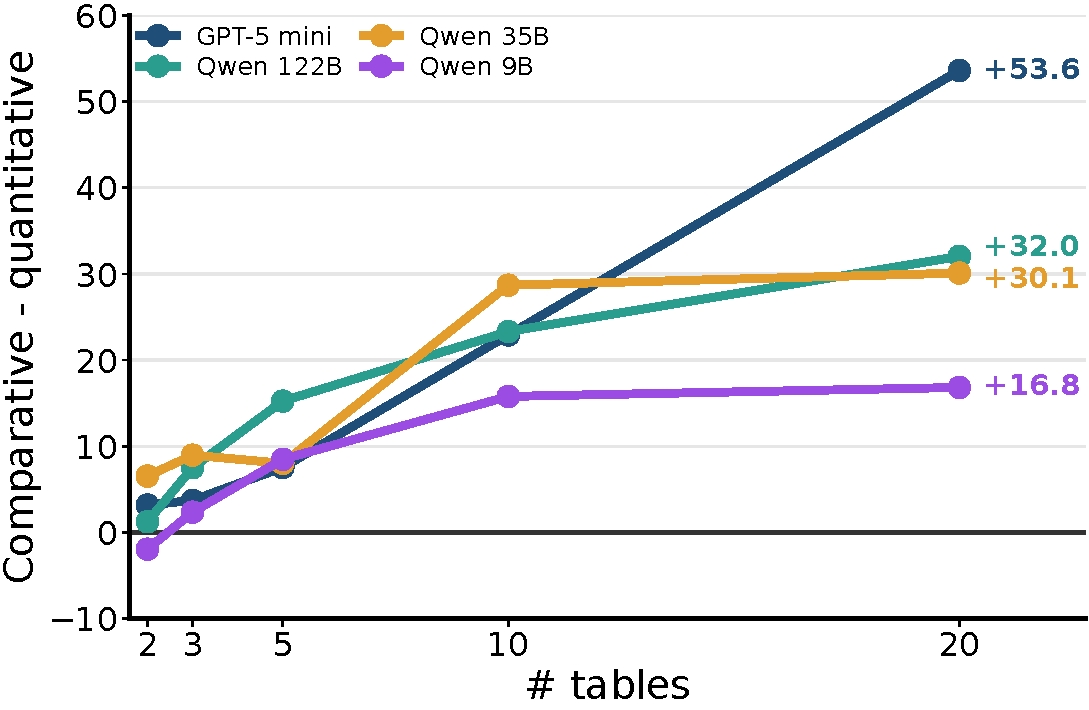
\includegraphics[width=\linewidth]{img/quant_vs_rel.pdf}
\caption{Performance gap between comparative and quantitative parallel questions as table count increases, averaged over domains and unit settings.
}
    \label{fig:question_type_gap}
\end{figure}
\stitle{(\textbf{RQ1}) Scaling collapses performance.}
As shown in \autoref{fig:scaling_parallel_sequential}, \emph{accuracy degrades sharply as the number of tables grows}, in both parallel and sequential regimes. For parallel questions, scaling from 2 to 20 tables costs \texttt{gpt-5-mini} 39.6 points, and Qwen 122B, 35B, and 9B 26.1, 32.8, and 38.3 points (\autoref{fig:parallel_scaling}). \texttt{gpt-5-mini} leads with few tables (95.53\% at 3) but collapses to 52.61\% at 20, where Qwen 122B, 35B, and 9B reach 64.90\%, 56.42\%, and 26.74\%. Sequential accuracy follows the same trend: extending the chain from 2 to 5 tables costs 32.5 points for \texttt{gpt-5-mini} and 28.8, 24.6, and 10.9 points for Qwen 122B, 35B, and 9B (\autoref{fig:sequential_scaling}). 
Additionally, \emph{sequential reasoning is harder than parallel aggregation.} Because it forces the model to propagate lookup keys across tables rather than combine independent evidence, sequential accuracy drops even faster per table, with the gap over parallel questions widening from 21.6 points at 2 tables to 40.1 at 5 (\autoref{fig:parallel_sequential_penalty}). The two regimes thus stress models differently: sequential chains are harder per table, whereas parallel questions scale to far more tables, where the collapse makes them comparably difficult.
\begin{figure}[t]
    \centering
    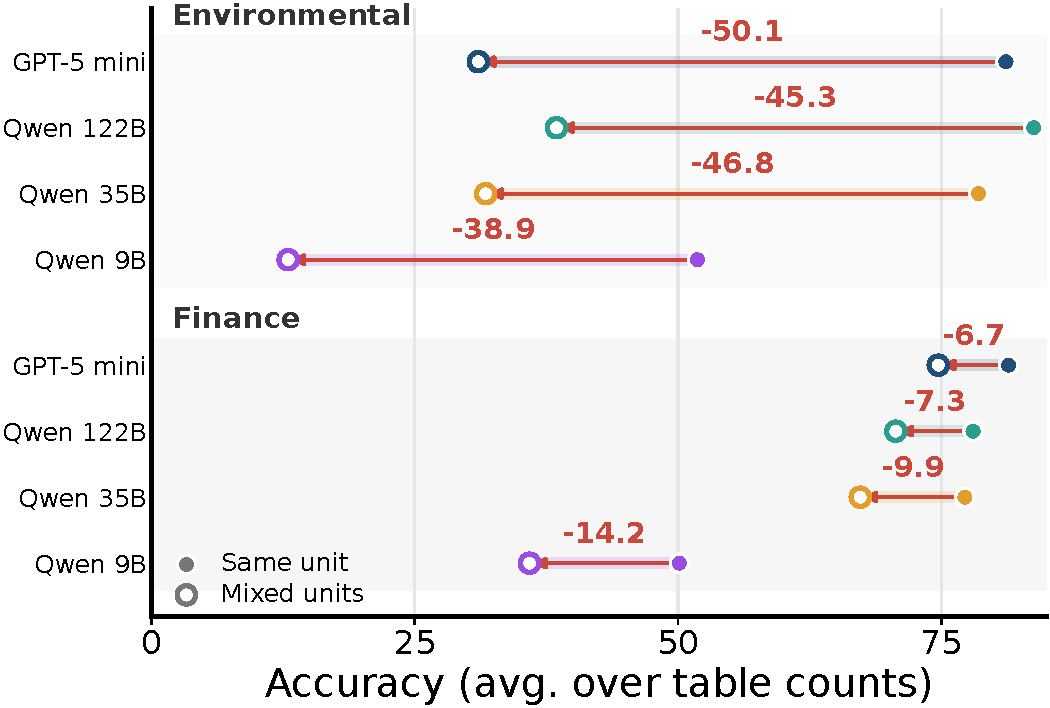
\includegraphics[width=\linewidth]{img/unit_heterogeneity.pdf}
    \caption{
    Per-model, per-domain accuracy drop from unit heterogeneity on parallel questions.
    }
    \label{fig:unit_heterogeneity}
\end{figure}
\stitle{(\textbf{RQ2}) Quantitative reasoning and unit heterogeneity are a major bottleneck.}
The scaling collapse is largely driven by precise numerical computation, as \emph{quantitative reasoning drives the collapse.} The gap between the accuracy over comparative and quantitative parallel questions widens with table count for every model (\autoref{fig:question_type_gap}): at 20 tables it peaks at 53.6 points for \texttt{gpt-5-mini}, and reaches 32.0, 30.1, and 16.8 points for Qwen 122B, 35B, and 9B, so quantitative questions account for a growing share of errors. This effect is amplified by unit heterogeneity, which causes \emph{a domain-dependent collapse.} As shown in \autoref{fig:unit_heterogeneity}, in the environmental domain, where questions often require physical conversions (e.g., gallons to liters), it costs \texttt{gpt-5-mini} 50.1 points and Qwen 122B, 35B, and 9B 45.3, 46.8, and 38.9, whereas in finance, dominated by scale conversions (e.g., thousands to billions), the same perturbation is far milder (6.7, 7.3, 9.9, and 14.2 points). 
Robustness to numerical representation is thus domain-specific, as each unit convention induce distinct failure modes~\cite{clariesg}.
\begin{table}[t]
\centering
\small
\setlength{\tabcolsep}{2.23pt}
\begin{tabular}{@{}l cc cc cc c@{}}
\toprule
\multirow{2}{*}{\textbf{Train data}} & \multicolumn{2}{c}{2} & \multicolumn{2}{c}{3} & \multicolumn{2}{c}{5} & \\
\cmidrule(lr){2-3}\cmidrule(lr){4-5}\cmidrule(lr){6-7}
& com & qnt & com & qnt & com & qnt & \textbf{Mean} \\
\midrule
None & 18.3 & 9.3 & 17.1 & 9.7 & 9.2 & 0.0 & 10.6 \\
\midrule
\name (fin) & 22.3 & 46.4 & 23.3 & 17.7 & 14.7 & 5.8 & 21.7$^{+11.1}$ \\
\name (env) & 35.5 & 50.0 & 35.3 & 18.3 & 25.8 & 5.0 & 28.3$^{+17.7}$ \\
\midrule
TAT-QA & 33.1 & 46.4 & 28.3 & 19.0 & 13.3 & 4.2 & 24.1$^{+13.5}$ \\
GRI-QA & 73.5 & 44.9 & 53.0 & 15.0 & 32.5 & 3.3 & 37.0$^{+26.4}$ \\
\midrule
\makecell[l]{\name (env)\\[-1pt]+ GRI-QA} & 83.5 & 52.9 & 70.0 & 15.0 & 48.1 & 12.5 & 47.0$^{+36.4}$ \\
\bottomrule
\end{tabular}
\caption{Accuracy of Qwen2.5-14B-Instruct fine-tuned on different training splits, evaluated on GRI-QA by number of tables and question type (comparative, quantitative), averaged over 3 seeds. Superscripts report the gain over the non-finetuned baseline; std. dev. in \S\ref{app:variance}.
}
\label{tab:finetuning}
\end{table}
\stitle{(\textbf{RQ3}) \name-generated data has functional utility.}
Beyond evaluation, we test whether \name-generated data is useful as training supervision by augmenting it with \texttt{gpt-5-mini} reasoning traces whose final answers match the SQL-derived gold answers, and fine-tuning \texttt{Qwen2.5-14B-Instruct}. 
We evaluate on GRI-QA~\cite{1.16}, which poses parallel comparative and quantitative questions over 2-, 3-, and 5-table environmental settings (\autoref{tab:finetuning}).
Since no comparable multi-table non-relational training set exists, which is the very gap \name targets, we compare against the three most relevant options: the in-domain GRI-QA train split, an out-of-domain single-table set (financial TAT-QA~\citealp{1.9}), and no fine-tuning. The TAT-QA baseline probes a common deployment scenario: a practitioner who needs a multi-table system in a target domain, but lacks in-domain multi-table data, falls back on an available single-table set from another domain. To keep the comparison fair given GRI-QA's limited size, every regime is capped at 440 instances, a cap that is itself a symptom of the data scarcity \name addresses.
All regimes improve over the non-finetuned baseline (+11.1 to +36.4 on average), and two takeaways emerge. First, \emph{in-domain multi-table supervision matters most.} Because both the domain and the reasoning structure of the training data align with the test setting, \name (env) leads out-of-domain TAT-QA at every table count, with the gap widening from +3.0 at 2 tables to +6.7 at 5. TAT-QA collapses as tables accumulate (8.8 average at 5 tables), while \name (env) degrades more gracefully (15.4). Second, \emph{\name complements scarce in-domain data.} As expected, GRI-QA leads \name (env) overall, since it is trained on the same distribution as the test set; however, GRI-QA's train split is skewed toward comparative questions ($\sim$3$\times$ more comparative than quantitative), so the GRI-QA-tuned model stays weak on quantitative reasoning compared to \name (env). Moreover, \name can cheaply supply the multi-table examples GRI-QA's split lacks: combining GRI-QA + \name (env) yields the best model overall (+36.4) and improves performance at \emph{every} table count and question type over GRI-QA alone. This confirms that \name augments rather than merely substitutes for real data, providing the scalable, multi-table supervision that existing benchmarks lack.
\stitle{(\textbf{RQ4}) Question generation is reliable.}
Question generation is the only \name stage that can introduce errors, since answers and evidence are guaranteed correct by construction. To estimate its reliability, we manually inspected 240 instances in the environmental and finance domain, 10 per aggregation operator (sum, average, superlative) across parallel (20 and 10 tables, unit-converted) and sequential (5 and 3 tables) regimes. Since we target the most error-prone settings, with many tables and unit conversions, reliability is likely higher in easier ones. 
\emph{Reliability is high}, as parallel instances average 99.2\%, while sequential ones 92.5\% (\autoref{tab:correctness}). The gap is expected, because sequential verbalization must coordinate constraints across heterogeneous tables rather than reuse a shared predicate. All errors trace to a dropped or hallucinated \texttt{WHERE} constraint, likely fixable with a stronger backbone than \texttt{gpt-5-mini}. Moreover, \emph{this reliability is competitive with manually curated benchmarks}: even in the hardest settings, 
\name's measured error rate stays below those reported for hand-built tabular datasets~\cite{5.8}, where error rates can reach up to 30\%. 
\begin{table}[t!]
\centering
\small
\setlength{\tabcolsep}{0.55em}
\renewcommand{\arraystretch}{1.2}
\begin{tabular}{l ccc c}
\toprule
& \multicolumn{2}{c}{\textbf{Quantitative}} & \textbf{Comparative} & \\
\cmidrule(lr){2-3} \cmidrule(lr){4-4}
\textbf{Topology} & \textit{Avg} & \textit{Sum} & \textit{Superlative} & \textbf{Mean} \\
\midrule
Parallel    & 100.0 & 100.0 & 97.5 & 99.2 \\
Sequential  &  95.0 &  87.5 & 95.0 & 92.5 \\
\midrule
\textbf{Mean} & 97.5 & 93.8 & 96.3 & 95.9 \\
\bottomrule
\end{tabular}
\caption{Manually verified correctness (\%) of \name-generated instances.}
\label{tab:correctness}
\end{table} 
